\documentclass[10pt]{article} % For LaTeX2e
\usepackage{tmlr}
% If accepted, instead use the following line for the camera-ready submission:
%\usepackage[accepted]{tmlr}
% To de-anonymize and remove mentions to TMLR (for example for posting to preprint servers):
%\usepackage[preprint]{tmlr}

\input{math_commands.tex}

\usepackage{hyperref}
\usepackage{url}
\usepackage{graphicx}
\usepackage{booktabs}
\usepackage{amsmath}
\usepackage{amssymb}
\usepackage{multirow}

\title{Input Pathways Shape Few-Shot, Not Zero-Shot, Binding in Tiny Transformers:\\
A Fully-Enumerable Study}

\author{\name Anonymous Author(s) \email anon@example.com \\
      \addr Anonymous Institution}

\newcommand{\microground}{\textsc{MicroGround}}

\def\month{MM}
\def\year{YYYY}
\def\openreview{\url{https://openreview.net/forum?id=XXXX}}

\begin{document}
\maketitle

\begin{abstract}
How does the \emph{way} information reaches a transformer---as symbolic in-context tokens, as a
clean per-factor ``oracle'' code, or as an entangled perceptual vector---affect whether the model
can \emph{bind} that information compositionally? We study this in a deliberately extreme regime:
transformers of $\sim$6--10K parameters on finite factored worlds that we enumerate exhaustively,
so every behavioral measurement is evaluated on the entire input space (zero sampling variance),
the informative input channels are matched in the sense that each uniquely determines the answer
(verified by exact Bayes ceilings), and every headline comparison is run at 10--20 seeds with
paired nonparametric tests (robustness arms use 5--20).
We report four findings. (1)~\emph{Endpoint invariance:} on held-out binding queries no informative
route yields converged zero-shot composition---each ends at or below chance despite an exact Bayes
ceiling of $1.0$, so within our bounded sweep (a ${\sim}25\times$ parameter increase, a $10\times$
learning-rate range, weight decay, and longer training) all routes converge to lookup-like solutions
despite information-sufficient inputs. (The ceiling certifies that the input determines the answer,
not that the held-out mapping is identifiable from a training objective for which lookup suffices.)
(2)~\emph{A two-factor account of few-shot binding:} when a small fraction of the held-out query
type is leaked into training, within the tested cells sample efficiency is best predicted by
(i)~\emph{input-pathway parameter sharing} (a shared projection transfers to unseen query types;
per-factor embedding tables do not) and (ii)~\emph{readability} of the code (a poorly readable
entangled code, whose raw linear decodability drops $0.95 \to 0.58$, has the worst pooled few-shot
performance and saturates far below the readable alternatives; a dimension-matched control and a
graded readability sweep---few-shot accuracy is monotone in decodability at fixed input
dimension---isolate readability from dimension). Two parameter-controlled pairwise dissociations (a three-cell
partial factorial) separate the factors; the two core effects (sharing helps, low readability hurts)
replicate across two held-out shape query types at 20 seeds, and are corroborated as a stress check
in a modestly larger three-object world, while the weak-perceptual edge over the oracle is testbed-specific. Notably, the clean per-factor oracle is not the most sample-efficient
readable route; shared readable pathways transfer better.
(3)~\emph{A double dissociation:} early in training, distributed codes---but not index-like
codes---pass through a transient phase of above-chance zero-shot transfer before collapsing into
memorization (clearly for the symbolic and weak-perceptual routes; the strong-entangled route's
collapse is comparable but its peak CI overlaps chance); this trajectory effect tracks code \emph{format}, whereas few-shot
efficiency tracks pathway \emph{sharing}. (4)~\emph{Failure anatomy:} the symbolic route fails by
\emph{losing} the answer at the readout position; index routes fail by \emph{systematically
mis-binding}---the answer stays decodable in the residual, yet a direct input intervention shows
the converged output is more sensitive to the \emph{wrong} object slot than to the correct one---and
the entangled route inherits, rather than improves on, the readability of its input.
Of these, the central positive claim is the two-factor account of few-shot efficiency; endpoint
invariance and failure anatomy are diagnostic constraints on it, and the transient a dynamical
correlate.
All code, manifests, and per-seed logs are available anonymously for exact reproduction.
\end{abstract}

\section{Introduction}
\label{sec:intro}
A transformer can receive the same fact in different ways. ``The object on the right is a square''
can arrive as words in the token stream, as a slot in a structured state vector, or as coordinates
of an entangled ``perceptual'' embedding. The symbol grounding debate
\citep{harnad1990symbol,bender2020climbing,bisk2020experience,merrill2021provable} asks whether the
non-symbolic routes confer something the symbolic route cannot; recent mechanistic work localizes
grounding-like mechanisms in language models \citep{wu2025mechanistic}, and a related line shows
that \emph{where} matched information is stored (weights versus context) changes how a transformer
generalizes from it \citep{chan2022transformers}. But these studies never hold the information
content of the routes constant: symbolic and perceptual conditions differ in dataset, model, and
difficulty, so route is confounded with everything else.

We ask the controlled version of the question. Fix a finite world of independent categorical
factors; deliver the \emph{same} state---provably sufficient to answer every query---through five
different input routes; and measure, exhaustively, what the model learns, how it learns it, and how
it fails. Our testbed, \microground{}, is small enough ($128$--$256$ states, $\sim$6--10K-parameter
transformers) that we can evaluate every model on the \emph{entire} query space, compute exact
Bayes-optimal ceilings per route, and probe every checkpoint. This trades scale for a property
larger studies cannot have: when a model fails, we can say \emph{exactly} whether the information
was absent, present-but-unread, or present-but-unusable, and when two routes differ, no sampling
noise or information mismatch can explain the difference. We therefore study \emph{information-matched
input encodings and pathways}, not grounding in the rich sense: the ``perceptual'' routes are fixed
synthetic codes of enumerated categorical states, and grounding is a motivating question, not a
claim we test.

Our target phenomenon is \emph{compositional binding}: answering ``shape of right'' requires
binding the queried attribute to the correct object slot \citep{greff2020binding,feng2024how}. We
hold out an entire query type (e.g., the model is never asked the shape of the right object during
training) and test whether each route composes the attribute concept, which it has seen, with the
object slot, which it has also seen. We complement binding with a systematic transformation task
(counterfactual successor, $v \mapsto (v{+}1) \bmod k$) under a transition holdout, an instance of
the leave-region-out diagnostic of \citet{hu2024case}.

An initially plausible hypothesis---that entangled, grounded-like routes encourage compositional
structure---is falsified here by a strong-entangled control (an entangled perceptual code that
defeats linear decoding), replicated across two held-out shape query types. What the controls isolate
instead is a mechanistic account of \emph{which properties of an input pathway matter, for what, and
why}, together with an unusually well-controlled negative result about zero-shot
compositionality at this scale.

\paragraph{Contributions.}
\begin{itemize}
\item \textbf{Testbed and method} (\S\ref{sec:testbed}--\S\ref{sec:ceilings}): \microground{},
fully-enumerable factored worlds with route-factored conditions (symbolic / factored-oracle /
weak- and strong-entangled perceptual / one-hot-shared, plus floor and scrambled controls), exact
per-route solvability ceilings, exhaustive evaluation with zero sampling variance, and a
statistical protocol (converged-accuracy metric, 5--20 seeds with 10--20 for all headline
comparisons, paired Wilcoxon with Holm--Bonferroni, bootstrap CIs, effect sizes) under an explicit
exploratory/confirmatory split.
\item \textbf{Endpoint invariance} (\S\ref{sec:endpoint}): no informative route achieves converged
zero-shot compositional binding; robust to capacity, weight decay, and training length; all failures
occur strictly below a ceiling of $1.0$, so the inputs are information-sufficient while the held-out
mapping is not identifiable from a training objective for which lookup suffices. (A transition-holdout
diagnostic shows the same memorization pattern; we treat it as weaker supporting evidence, as the
tiny world may not reward the rule.)
\item \textbf{A two-factor account of few-shot binding} (\S\ref{sec:fewshot}): within the tested
cells, two pairwise dissociations point to input-pathway parameter sharing and practical readability
as the dominant predictors of sample efficiency (a three-cell partial factorial, not a full
interaction estimate); the clean per-factor oracle is not the most sample-efficient readable route;
the effects replicate across two held-out shape query types at 20 seeds and are corroborated as a
stress check in a modestly larger three-object world, and are robust to description order, synthetic
mix, and---for readability---a dimension-matched control.
\item \textbf{A double dissociation} (\S\ref{sec:dynamics}): transient zero-shot transfer early in
training tracks code format (distributed vs.\ index-like); few-shot efficiency tracks pathway
sharing. Exhaustive evaluation makes the transient a measured behavioral state, not noise.
\item \textbf{Failure anatomy} (\S\ref{sec:anatomy}): control-task probes plus a causal
input-intervention separate three failure modes---representation death at the readout position
(symbolic), systematic mis-binding with the answer decodable but the output depending, under input
intervention, on the wrong slot (index routes), and no readability gained over the input (entangled route).
\end{itemize}

\section{Related Work}
\label{sec:related}
\paragraph{Mechanistic symbol grounding.} Closest to our framing, \citet{wu2025mechanistic} train
transformers and SSMs from scratch on a testbed where each lexical item has an environmental token
and a linguistic token, quantify grounding as the surprisal reduction of the linguistic token given
a \emph{matched} versus \emph{mismatched} referent, and localize a middle-layer ``aggregate''
attention mechanism. Their manipulation is referent correctness (matched vs.\ mismatched referent
within a from-scratch token testbed, with a multimodal-dialogue replication), not \emph{route}, and
the conditions are never information-matched, so a similarity between conditions cannot separate
route from modality difficulty. Holding information constant across routes is exactly our
manipulation---and our falsified hypothesis (\S\ref{sec:fewshot}) shows why the control matters.

\paragraph{Where information is stored, and how it is encoded.} \citet{chan2022transformers} show,
via a partial-exposure paradigm, that matched information generalizes rule-like from weights but
exemplar-like from context. We fix the storage locus (all state routes are in-context side-channels)
and vary the \emph{encoding} instead; but the connection is more than orthogonality: their
context$\to$exemplar bias arguably \emph{predicts} our endpoint invariance (all in-context routes
collapse to memorization, \S\ref{sec:endpoint}), which we take as convergent support for the
inductive-bias reading rather than an independent finding. That the \emph{form} of an encoding
governs generalization is also known on other axes---most directly positional-encoding choice and
length generalization \citep{kazemnejad2023impact}---and compositional generalization has a
standing taxonomy \citep{hupkes2020compositionality}; our contribution is an information-matched
route manipulation with exact ceilings, not the bare claim that encoding matters.

\paragraph{Rule versus memorization.} \citet{hu2024case} introduce leave-region-out diagnostics on
arithmetic grids and show GPT-2-scale transformers reason case-based rather than rule-based; our
transition holdout is a direct instance of their diagnostic, which we credit as the method. Our
contribution there is the route comparison and the exact-ceiling framing (models fall below even
the blind-majority bound). Grokking work \citep{power2022grokking,nanda2023progress,zhong2023clock}
motivates our weight-decay arm, which fails to induce rule learning here (\S\ref{sec:endpoint}).

\paragraph{Binding.} \citet{feng2024how} characterize the additive Binding-ID mechanism by which
large language models bind entities to attributes in context; their setting is purely symbolic.
\citet{greff2020binding} frame binding as a core representational problem. We study the same
computational problem at a scale where the full input space is enumerable and ask how the binding
substrate depends on the input pathway.

\paragraph{Exact bounds and toy-model interpretability.} \citet{gross2024compact} prove
computer-assisted \emph{lower} bounds on a specific trained model's accuracy, priced by the
compactness of its circuit; Tracr \citep{lindner2023tracr} compiles known circuits. Our solvability
analysis is a different object: model-agnostic \emph{upper} bounds (Bayes ceilings) computed a
priori from the enumeration, used to classify failures as information- versus inductive-bias-driven.

\paragraph{World models, compositional generalization, and encodings.} Emergent world
representations are probed and edited in task-defined worlds \citep{li2023emergent}; grounded
compositional benchmarks \citep{lake2018generalization,ruis2020benchmark,kim2020cogs} are large and
behavior-only. Two prior results are especially close and temper our positive claims. First,
architectural weight/parameter \emph{sharing} is known to aid systematic generalization
\citep{csordas2021devil}; our pathway-sharing factor is an information-matched, exactly
parameter-matched instance of this, not a fresh discovery. Second, \citet{montero2021role} show
that disentangled representations, even when handed to the model, are \emph{not sufficient} for
harder compositional generalization---the direct precedent for our ``clean oracle is worst''
result; we contribute a candidate mechanism (pathway sharing) for why. Our finding that models
exploit linearly-readable features and fail to disentangle further connects to shortcut learning
and simplicity bias \citep{geirhos2020shortcut,shah2020pitfalls,hermann2020shapes} (with the
caveat that readability here \emph{helps} rather than names a failure mode) and to the difficulty
of unsupervised disentanglement \citep{locatello2019challenging}; our probes follow the control-task methodology of
\citet{hewitt2019designing}, with representation geometry in mind \citep{elhage2022toy}. Grounding
debate anchors \citep{bender2020climbing,bisk2020experience,merrill2021provable,patel2022mapping}
motivate the operational question without settling it.

\paragraph{What is isolated here, versus already known.} Individually, several ingredients are not
new: parameter sharing aids systematic generalization \citep{csordas2021devil}, disentangled codes
are not sufficient for it \citep{montero2021role}, and small transformers memorize under weak
compositional pressure. Our contribution is not any single effect but the \emph{confound removal}
that lets these be separated: by matching information exactly (verified by per-route Bayes
ceilings), enumerating the entire input space, and factoring the input pathway into sharing, code
format, and readability, we isolate variables that modality comparisons ordinarily leave entangled
with dataset, capacity, difficulty, and information content.

\section{The \microground{} Testbed}
\label{sec:testbed}
\paragraph{Worlds.} The single-object world has four independent categorical factors (colour,
shape, position, size) of cardinalities $(4,4,4,2)$: $128$ states. The two-object world places two
objects in fixed positional roles (left, right), each with a colour and a shape: $4^4 = 256$
states. Both worlds are enumerated in full; every evaluation below is over the \emph{entire}
relevant query space, so for a fixed split and trained model, evaluation has zero sampling variance;
across the reported runs, variance comes from model initialization and, where applicable, the split
or leakage seed.

\paragraph{Tasks.} \emph{Attribute} (report a queried factor; a lookup used as a sanity ceiling),
\emph{counterfactual} (report the successor $(v{+}1) \bmod k$ of a queried factor), and
\emph{binding} (report one attribute of the object at a queried position, e.g.\ ``shape of
right''). The two-object binding task has four query types, one per (position, attribute) pair,
$256$ queries each.

\paragraph{Routes (conditions).} A condition factors into a text form and a state encoder, so the
same exhaustive query set is realized under every route. The five informative routes each uniquely
determine the answer (verified in \S\ref{sec:ceilings}); the two floors
(\texttt{text\_minimal}, \texttt{uninformative\_state}) provide none of the state, and
\texttt{scrambled\_state} is an information-matched control code. The same exhaustive query set is
realized under every route (Table~\ref{tab:routes}).
\begin{table}[h]
\centering\footnotesize
\resizebox{\textwidth}{!}{%
\begin{tabular}{llll}
\toprule
Condition & Input & State channel & Raw linear dec.\\
\midrule
\texttt{text\_only} (symbolic) & description + question & --- & (in tokens)\\
\texttt{state\_factored} (oracle) & question & per-factor index $\to$ per-factor emb.\ tables & indices\\
\texttt{state\_onehot\_shared} & question & concat.\ one-hot $\to$ shared linear & $1.0$\\
\texttt{state\_perceptual} (weak) & question & fixed 2-layer tanh mix, $d{=}16$ $\to$ shared linear & $0.95$\\
\texttt{state\_perceptual\_hard} & question & fixed 3-layer tanh mix, $d{=}8$, gain $2.5$ $\to$ shared linear & $0.58$\\
\midrule
\texttt{text\_minimal} (floor) & question & --- & ---\\
\texttt{uninformative\_state} (control) & question & constant vector & ---\\
\texttt{scrambled\_state} (control) & question & fixed bijective relabeling & indices\\
\bottomrule
\end{tabular}}
\caption{Routes. ``Raw linear dec.'' is 5-fold logistic decoding of a factor from the raw state
input (mean over factors). The one-hot-shared and weak-perceptual routes use an identical
$16{\to}24$ linear input pathway (exactly matched parameter count); the factored oracle uses
per-factor embedding tables of nearly identical total size. The perceptual mixes are fixed
(run-independent), so they are a shared ``perception,'' not trainable preprocessing. We use
``perceptual'' descriptively: \texttt{state\_perceptual} is a synthetic entangling map standing in
for a distributed non-symbolic code, not a learned or naturalistic perception. Our claims are about
input encodings and pathways; grounding is motivation, not a claim.}
\label{tab:routes}
\end{table}

\paragraph{Generalization splits.} Beyond random $80/20$ splits we use: \emph{binding holdout}
(remove an entire (position, attribute) query type from training; test on all $256$ of its
queries), \emph{$k$-shot binding} (leak a fraction $f$ of the held-out type back into training;
test on the rest), and \emph{transition holdout} (remove a random $30\%$ of (factor, source-value)
successor transitions; after \citealp{hu2024case}). Splits partition states or query types; query
generation is otherwise exhaustive and deterministic. The model is a 1-layer (2-layer in the
capacity arm) pre-norm transformer, hidden size $24$ ($\sim$6--10K parameters), trained with AdamW;
the state embedding is added to every token position.

\section{Protocol: Exhaustive, Converged, and Replicated}
\label{sec:protocol}
Three methodological choices matter for everything below. \textbf{(i) Converged, not peak.} We
report the \emph{converged} test accuracy (mean over the last $10\%$ of evaluations). During
exploration we found that the peak over training inflates transient generalization spikes that
decay by convergence (\S\ref{sec:dynamics} turns this artifact into an object of study); flat
controls (collapse $= 0.000$) rule out max-of-noise inflation. \textbf{(ii) Balanced accuracy with
baselines.} The primary metric is balanced accuracy (mean over per-query-type accuracy), always
reported against the chance and majority baselines; because evaluation is exhaustive, both are
exact. \textbf{(iii) Replication discipline.} Initialization and split seeds are separated; headline
results use $10$--$20$ seeds (robustness arms $5$--$20$) with bootstrap $95\%$ CIs, paired
Wilcoxon signed-rank tests across seeds, Holm--Bonferroni correction, and Cliff's $\delta$. Effects discovered during exploration (on
held-out type ``shape of right,'' \texttt{bind:3}) were re-tested at 20 seeds and then replicated
on a fresh held-out type (``shape of left,'' \texttt{bind:1}) with all routes run once,
confirmatory-style; we mark exploratory versus confirmatory results throughout. Every run appends
a self-describing record (config, seeds, trajectories) to a JSONL manifest from which all tables
and figures re-aggregate without retraining.

Two scope notes on the statistics. \emph{Interpreting null endpoint differences.} The endpoint-invariance
and no-transition-difference claims are acceptances of the null; we read them as bounded (``no knob
in this box''), and note that the paired zero-shot route-difference confidence intervals are smaller
than the $+0.05$--$0.08$ few-shot effects in Table~\ref{tab:fewshot}; we therefore treat endpoint
invariance as a bounded empirical observation, not a formal
equivalence claim.
\emph{The mechanism arms use $n{=}10$}; their effect sizes are large ($|\delta|\ge0.6$, $p<10^{-3}$)
and the one place a small effect mattered---the k-shot ordering---is exactly where our $10\to20$-seed
firm-up caught and shrank it, so we trust the large mechanism effects at $n{=}10$ while reporting the
smaller ones (symbolic route) as non-significant.

Two exploratory refinements did not survive this protocol. A three-way
route ordering visible at 10 seeds shrank to a two-group structure at 20 seeds; and our headline
hypothesis---that a grounded side-channel induces compositional structure---was falsified by the
strong-entangled control we designed to test it (\S\ref{sec:fewshot}).

\section{Exact Solvability Ceilings}
\label{sec:ceilings}
Because the worlds are finite we compute, for every (task, split, route), the Bayes-optimal
balanced accuracy on the test queries: group test queries by exact input identity---two states
yield the same group only if their input vectors are identical, an injectivity check over the
finite enumeration---and predict the within-group majority. This is an a priori, model-agnostic
\emph{upper} bound on any learner's test behavior \emph{given the input}---a channel property, to
be contrasted with proof-based \emph{lower} bounds for specific trained networks
\citep{gross2024compact}. Two things it does \emph{not} certify: that the mapping is identifiable
from \emph{training} (for a held-out query type it is not), and that the input is easy for a
particular decoder or model class to read.

The audit yields three facts used throughout. (1)~Every informative route is \emph{injective}
(ceiling $1.0$) on every split: distinct states yield distinct inputs, so no informative route below fails for
lack of information in the input---failures are of inductive bias or (for held-out query types)
train-time identifiability, not of channel capacity. (2)~The floors are exactly chance on binding
holdouts (ceiling $0.250$: the question alone carries nothing) and $0.833$ on transition holdouts
(held-out transitions have degenerate target distributions a blind majority guesser can exploit).
(3)~The controls behave as designed: \texttt{uninformative\_state} tracks \texttt{text\_minimal}
everywhere (e.g., $0.296$ vs.\ $0.296$ peak on the random-split counterfactual task; Cliff's
$\delta = +0.02$), and \texttt{scrambled\_state} reaches $1.000$ in distribution---an arbitrary
bijective code is learned perfectly when information content is matched. Full ceiling values are
in Appendix~\ref{app:ceilings}.

\section{Results I: Endpoint Invariance---No Route Yields Zero-Shot Compositionality}
\label{sec:endpoint}
\paragraph{Binding.} Table~\ref{tab:zeroshot} gives converged accuracy on the held-out query type
(exploratory holdout, $n{=}20$). Every route ends at or below chance ($0.25$); the strong-entangled
route ends far below ($0.146$), and the oracle ends below ($0.198$)---systematic error, not
agnosticism (\S\ref{sec:anatomy}). In-distribution learning is intact (all informative routes fit
the three trained query types; random-split sanity checks confirm the models learn the task in
distribution), so the failure is specific to composition. \textbf{Scope.} Because training
covers three of the four query types, pure lookup is a low-loss training solution, so the world
does not strongly \emph{reward} composition; ``endpoint invariance'' should be read as ``in
training regimes where memorization suffices, no informative route within our bounded sweep (${\le}2$ layers,
${\le}96$ hidden, AdamW, LR/wd ranges below, ${\le}4000$ epochs) escapes it,'' not as a universal
limit. The exact ceiling of $1.0$ rules out an \emph{information} explanation, not a
training-objective one; a design that makes lookup costly (more held-out types) is the right next
test and is future work.

\begin{table}[h]
\centering\small
\begin{tabular}{lccc}
\toprule
Route & Converged held-out acc.\ [95\% CI] & Peak (transient) & Collapse\\
\midrule
\texttt{text\_minimal} (floor) & 0.237 [0.21, 0.25] & 0.237 & 0.000\\
\texttt{uninformative\_state} & 0.237 [0.21, 0.25] & 0.237 & 0.000\\
\texttt{text\_only} & 0.227 [0.19, 0.26] & \textbf{0.358} [0.33, 0.39] & \textbf{0.131} [0.09, 0.18]\\
\texttt{state\_factored} & 0.198 [0.16, 0.23] & 0.224 & 0.026\\
\texttt{state\_onehot\_shared} & 0.215 [0.20, 0.23] & 0.249 & 0.034\\
\texttt{state\_perceptual} & 0.224 [0.20, 0.24] & \textbf{0.308} [0.29, 0.33] & 0.084 [0.06, 0.12]\\
\texttt{state\_perceptual\_hard} & 0.146 [0.11, 0.18] & 0.286 [0.24, 0.33] & \textbf{0.140} [0.10, 0.19]\\
\bottomrule
\end{tabular}
\caption{Zero-shot compositional binding (held-out query type ``shape of right''), $n{=}20$ seeds,
chance $= 0.250$, ceiling of every informative route $= 1.0$. No route generalizes at convergence;
the transient peaks and collapses are analyzed in \S\ref{sec:dynamics}.}
\label{tab:zeroshot}
\end{table}

\paragraph{Transitions.} On the counterfactual successor task with $30\%$ of transition types held
out, every route converges to $0.000$--$0.058$ on held-out transitions (weak-perceptual exactly
$0.000$; no significant route differences, Holm $p \ge 0.72$; $n{=}10$; the training set is fully
memorized, all-space balanced accuracy $0.69$--$0.75$, flat for the last $960$ of $1000$ epochs).
Note that even the best of these, $0.058$, falls far below $0.833$: every route is worse than a
blind majority guesser---the models do not abstain but emit systematically wrong answers. We
caution, however, that with only three visible transitions per factor the world may not
\emph{reward} the successor rule at all; we read the transition result as memorization under weak
compositional pressure, not as proof of a deep inductive-bias pathology, and do not lean on it
beyond the binding conclusion.

\paragraph{Robustness.} The invariance is not a budget artifact. \emph{Capacity:} at hidden sizes
$24\to48\to96$ and $1\to2$ layers ($6$K$\to$$21$K$\to$$40$K$\to$$153$K parameters, ${\sim}25\times$),
converged held-out binding stays at
or below chance for every route swept (symbolic, oracle, weak-perceptual); capacity instead
softens the failure's distinctive character (the oracle's below-chance converged accuracy rises
from $0.178$ to $0.240$, approaching chance; the symbolic transient peak decays $0.385 \to 0.258$
in the $n{=}8$ capacity arm, cf.\ $0.358$ at $n{=}20$ in Table~\ref{tab:zeroshot}).
\emph{Learning rate:} at $3\times10^{-4}$ and $3\times10^{-3}$ ($10\times$ around the default),
converged held-out binding remains $0.18$--$0.24$ for all three routes tested ($n{=}10$).
\emph{Regularization:} on the oracle route, weight decay $\in \{0.01, 0.1, 0.3, 1.0\}$ for
$4{,}000$ epochs ($\approx$52K steps) leaves held-out transition accuracy at $0.000$ in every
cell---the regularizer that reliably induces grokking in modular arithmetic at this parameter
scale does nothing here, consistent with the successor task's lack of compressive coupling across
values, and with a world (three visible transitions per factor) that may simply be too small to
reward the rule. \emph{Duration:} trajectories are flat long before evaluation ends. Grid details
are in Appendix~\ref{app:robust}.

\section{Results II: The Transient Compositional Phase Tracks Code Format}
\label{sec:dynamics}
Because evaluation is exhaustive, each point of a test trajectory is an exact property of the
network at that epoch. Early in training---and only early---some routes pass through a state of
genuine zero-shot transfer to the never-trained query type (Table~\ref{tab:zeroshot}, ``peak'';
Figure~\ref{fig:dynamics}): the symbolic route reaches $0.358$ [0.33, 0.39] around epoch 12 and the
perceptual routes reach $0.286$--$0.308$ (the strong-entangled peak's CI overlaps chance), before
all collapse into memorization. The two index-like
routes never leave chance (peaks $0.22$--$0.25$), and the flat floors (collapse exactly $0.000$)
exclude max-of-noise explanations.

Collapse magnitude separates routes sharply: \texttt{text\_only} vs.\ \texttt{state\_factored}
$p_{\text{adj}} = 7.8\times10^{-4}$, $\delta = +0.71$; \texttt{state\_factored} vs.\
\texttt{state\_perceptual} $p_{\text{adj}} = 9.0\times10^{-4}$, $\delta = -0.64$, i.e.\ the oracle
collapses less (Holm-corrected paired Wilcoxon, $n{=}20$). The grouping is by \emph{code format}---here, whether the queried attribute enters as a
distributed continuous vector or token sequence (\texttt{text\_only}, weak and strong perceptual
mixes) versus a discrete slot index (\texttt{state\_factored}, and \texttt{state\_onehot\_shared},
whose one-hot is a single active index): the token and weak-perceptual distributed codes transiently
support composition, while the hard-perceptual route shows a comparable collapse but only a weaker
peak whose CI overlaps chance; the index-like codes go directly to lookup. Notably this grouping is \emph{different}
from the one that governs few-shot efficiency below---a double dissociation: trajectory shape
tracks format, few-shot efficiency tracks pathway sharing. The transient is also capacity-fragile
(the $n{=}8$ capacity-arm peak decays $0.385 \to 0.258$ from 6K to 153K parameters; cf.\ the
$n{=}20$ Table~\ref{tab:zeroshot} value $0.358$ at 6K), suggesting small models linger in a
shared-feature regime that larger ones skip.

\begin{figure}[t]
\centering
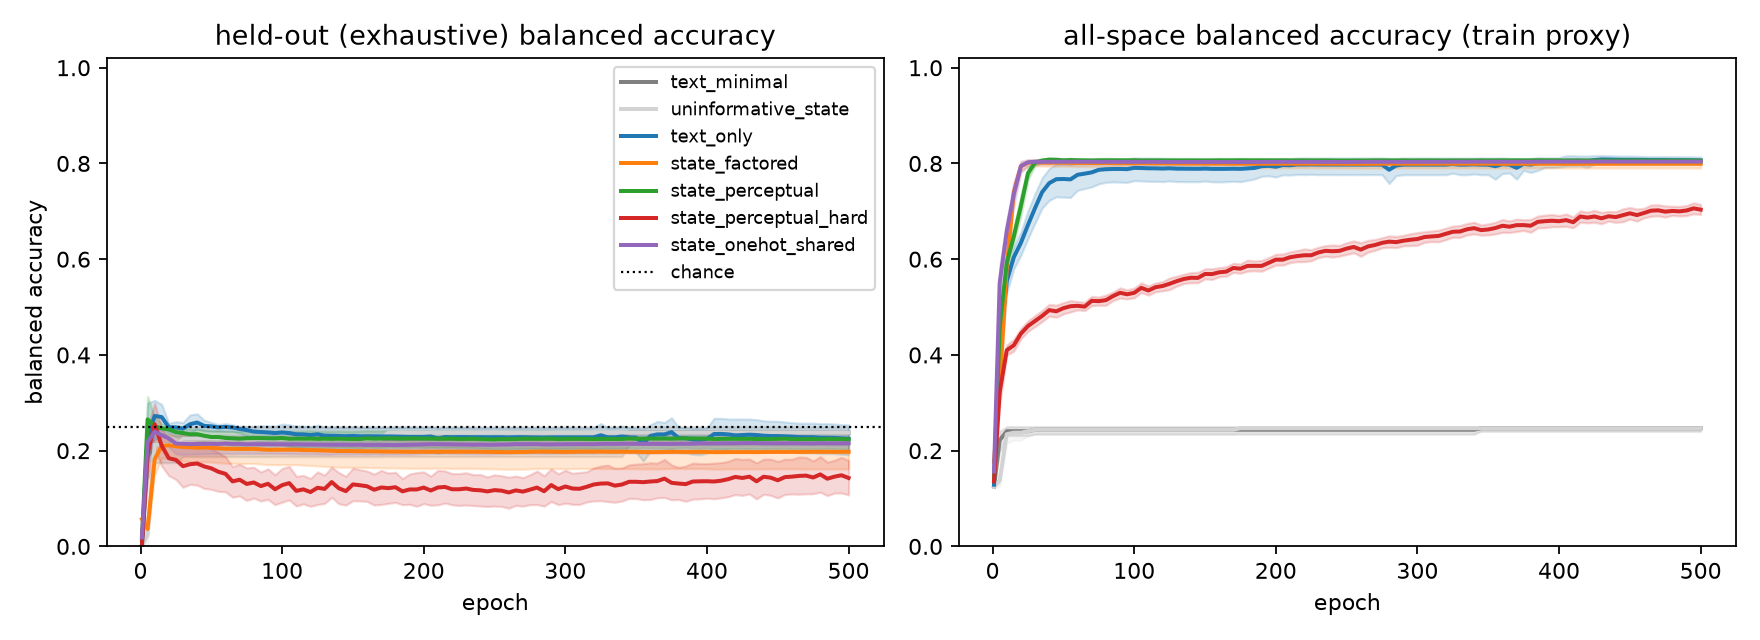
\includegraphics[width=0.98\textwidth]{figs/bind_holdout_route_dynamics.png}
\caption{Training dynamics by route on the held-out binding type ($n{=}20$ seeds; bands are
bootstrap 95\% CIs; every point is an exhaustive evaluation). Left: held-out (never-trained) query
type; the token and weak-perceptual distributed codes (blue/green) pass through a transient
above-chance phase and collapse (the hard-perceptual route, red, collapses comparably but its peak
CI overlaps chance);
index-like codes (orange/purple) and floors never rise above chance. Right: all-space accuracy (train
proxy) shows all informative routes memorize the trained types.}
\label{fig:dynamics}
\end{figure}

\section{Results III: Failure Anatomy---Where the Answer Goes}
\label{sec:anatomy}
For each route we retrained models with mid-training checkpoints ($n{=}10$) and measured, on the
held-out type: behavioral accuracy; the \emph{mis-binding rate} (among states whose left and right
shapes differ, the probability that the model answers with the \emph{left} shape); and a 5-fold
linear probe decoding the correct (right) shape from the final-token residual, with a
control-task probe \citep{hewitt2019designing} subtracted (selectivity $=$ probe $-$ control);
see Table~\ref{tab:anatomy}.

\begin{table}[h]
\centering\small
\begin{tabular}{lcccc}
\toprule
Route (converged) & Behav. & Mis-binding & Probe & Selectivity\\
\midrule
\texttt{text\_only} & 0.241 & 0.510 & 0.278 & $-0.013$ (0.215 at ep5)\\
\texttt{state\_factored} & 0.178 & 0.706 & \textbf{0.952} & 0.687\\
\texttt{state\_onehot\_shared} & 0.217 & \textbf{0.866} & \textbf{0.953} & 0.685\\
\texttt{state\_perceptual} & 0.173 & 0.431 & \textbf{0.963} & 0.682\\
\texttt{state\_perceptual\_hard} & 0.141 & 0.314 & 0.589 & 0.316\\
\bottomrule
\end{tabular}
\caption{Failure anatomy on the held-out binding type ($n{=}10$; chance behav.\ $=0.25$; probe
chance $=0.25$). Three modes: the symbolic route \emph{loses} the answer at the readout position
(selectivity $0.215$ at epoch 5, coinciding with its behavioral transient, decaying to $\approx 0$);
index routes keep the answer perfectly decodable yet systematically read the wrong slot; the
strong-entangled route's residual decodability ($0.589$) matches its \emph{raw input's} linear
decodability ($0.58$)---the model adds no disentanglement.}
\label{tab:anatomy}
\end{table}

\begin{figure}[t]
\centering
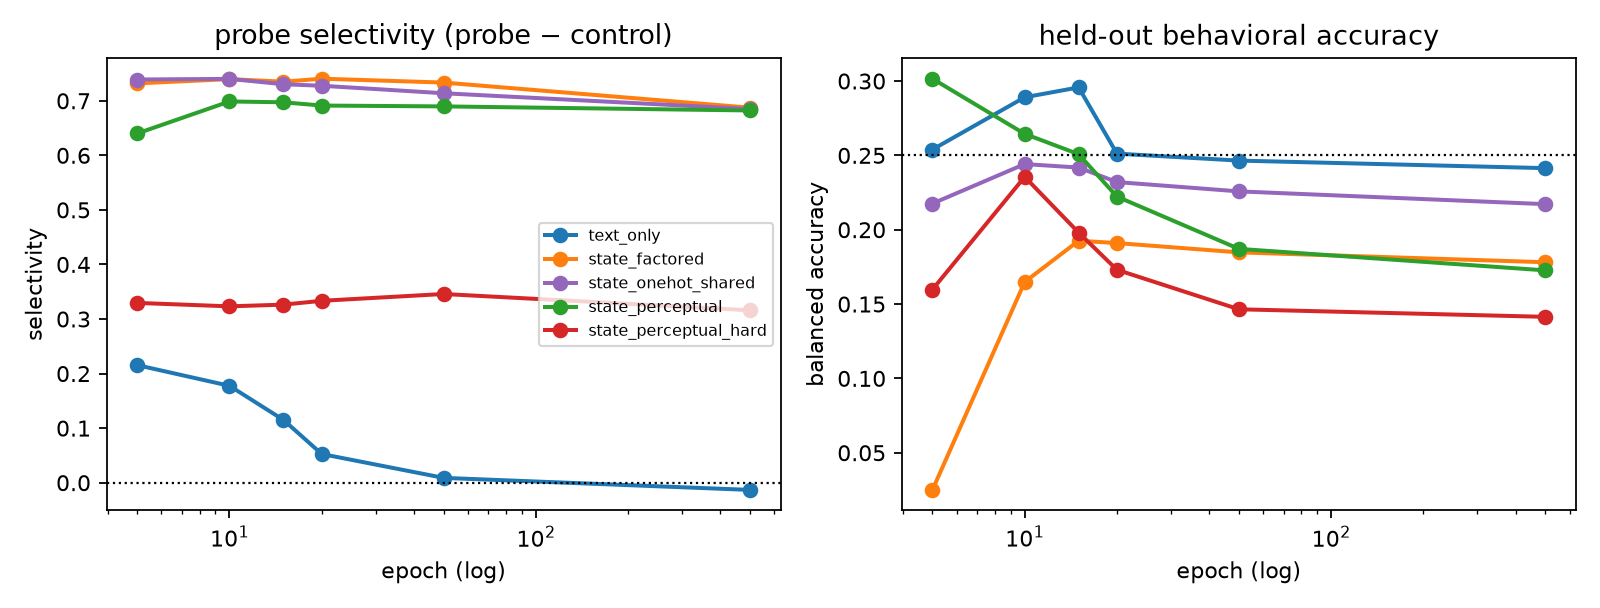
\includegraphics[width=0.9\textwidth]{figs/bind_probe_anatomy.png}
\caption{Failure anatomy across training ($n{=}10$; log-scale epochs; the last point is the
converged model). Left: control-subtracted probe selectivity for the correct held-out attribute at
the readout position. Right: held-out behavioral accuracy. The symbolic route (blue) briefly
represents the answer exactly while it briefly uses it, then loses both; index routes
(orange/purple) keep the answer decodable throughout while behavior stays at or below chance; the
entangled route (red) is pinned near its input's raw linear readability.}
\label{fig:anatomy}
\end{figure}

Three distinct failure modes emerge (Figure~\ref{fig:anatomy}). \emph{Representation death}
(symbolic): the answer is weakly
present at the readout position exactly while the behavioral transient lasts, then fades;
converged behavior is near-unbiased guessing among shapes. \emph{Systematic mis-binding} (index
routes): the answer remains near-perfectly linearly decodable in the residual stream at every
checkpoint, yet the converged model reads the wrong slot on up to $87\%$ of discriminating states---an intact representation but a behavioral output that depends on the wrong slot, the mechanistic ground of the
below-chance entries in Table~\ref{tab:zeroshot}. \emph{No readability gained} (strong-entangled):
residual decodability ($0.589$) equals the input's raw decodability at every checkpoint; the model
inherits its input's readability rather than improving on it. (We stop short of ``the information
is present but unused'': the strong code is injective---exact ceiling $1.0$, \S\ref{sec:ceilings}---so
no information is lost, but a nonlinear MLP decoder still recovers its factors at only $0.56$ from
the enumerated states, so it is hard for the decoder \emph{and} model classes we test, not merely
for a linear probe.)

\paragraph{From decodable to causal.} Probes show \emph{what is present}, not \emph{what is used}.
We therefore intervene directly on the world state and read the output (Table~\ref{tab:causal}). On
the held-out ``shape of right'' query, varying the correct (right) slot leaves the output almost
unchanged (all routes $0.15$--$0.24$, i.e.\ chance), while varying the wrong (left) slot moves it
strongly (index routes $0.71$--$0.86$; symbolic $0.51$)---the converged output is more sensitive to
the wrong object. As a positive control, on a \emph{trained} query type the same intervention shows
every route showing substantially greater causal dependence on the queried slot ($0.67$--$1.00$)
than on the unqueried one ($\approx 0.25$). What the intervention adds over the probe is real but bounded: it rules out
``decodable-but-causally-inert'' and shows the output functionally depends on the wrong slot under
input intervention, with the answer-representation intact. It identifies the functional readout the converged model uses: it
reuses the readout for the trained shape slot rather than the held-out one (holding out ``shape of
left'' instead flips which slot is read). The claim is the intact-representation-but-wrong-slot-dependence
dissociation, not the direction of the error.

\begin{table}[h]
\centering\small
\begin{tabular}{lcc|cc}
\toprule
& \multicolumn{2}{c|}{Held-out ``shape of right''} & \multicolumn{2}{c}{Trained ``shape of left''}\\
Route & vary right (correct) & vary left (wrong) & vary left (correct) & vary right\\
\midrule
\texttt{text\_only} & 0.24 & 0.51 & 1.00 & 0.25\\
\texttt{state\_factored} & 0.18 & 0.71 & 1.00 & 0.25\\
\texttt{state\_onehot\_shared} & 0.22 & \textbf{0.86} & 1.00 & 0.25\\
\texttt{state\_perceptual} & 0.17 & 0.43 & 0.67 & 0.26\\
\texttt{state\_perceptual\_hard} & 0.15 & 0.30 & 0.89 & 0.25\\
\bottomrule
\end{tabular}
\caption{Causal input-intervention on the held-out binding type ($n{=}10$; chance $0.25$). Each
number is the fraction of (background, value) cases in which the output equals the shape set in the
varied slot. On the held-out query the output is insensitive to the correct slot and, especially for
the index routes, depends more on the wrong slot; on a trained query it depends much more on the
queried slot than on the unqueried one---a direct manipulation of the input, with no probe
assumptions.}
\label{tab:causal}
\end{table}

\section{Results IV: A Two-Factor Account of Few-Shot Binding}
\label{sec:fewshot}
Zero-shot composition fails everywhere, but the cliff is informative once graded: we leak a
fraction $f \in \{0.02, 0.05, 0.1, 0.2\}$ of the held-out query type into training and measure
converged accuracy on the rest (Figure~\ref{fig:dose}). All readable routes rise smoothly from chance to
$0.82$--$0.96$ at $f{=}0.2$, while the strong-entangled route saturates near $0.48$; the question
becomes \emph{which pathway properties govern the rate}.

\begin{figure}[t]
\centering
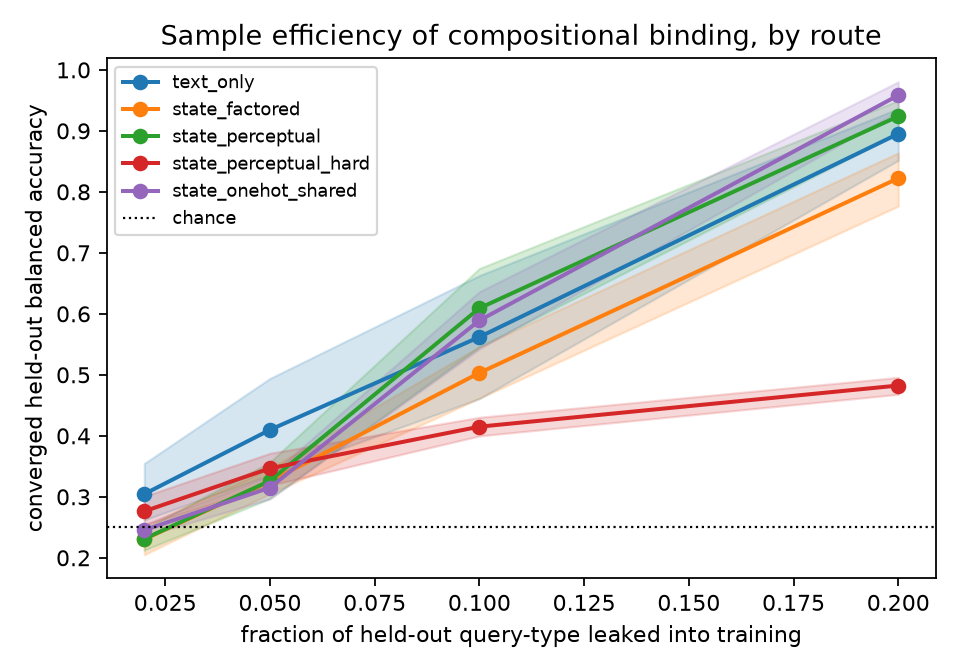
\includegraphics[width=0.62\textwidth]{figs/bind_doseresp.png}
\caption{Dose-response of compositional binding ($n{=}20$ seeds, converged accuracy, exploratory
holdout; bands are bootstrap 95\% CIs). The shared-pathway readable routes (blue, green, purple)
outperform the modular oracle (orange); the entangled route (red) saturates far below everything.}
\label{fig:dose}
\end{figure}

\paragraph{Entanglement does not explain few-shot transfer.} We initially hypothesized that \emph{entangled} routes
induce compositional structure (the model must compute factors, so it builds factorized machinery
that transfers). The strong-entangled route is this hypothesis's adversarial test: if entanglement
drives composition, harder entanglement should help. It does the opposite---worst pooled over doses,
saturating near $0.48$ while every readable route keeps rising past $0.82$; pooled disadvantage
vs.\ the oracle $-0.090$, $p = 3.8\times10^{-6}$ (exploratory) and $-0.112$, $p = 5.7\times10^{-6}$
(confirmatory). Is the strong code's information merely linearly hidden? No: a nonlinear MLP
decoder recovers its factors at only $0.56$ from the enumerated states (vs.\ $0.95$/$0.98$ linear/MLP
for the weak code), so the $d{=}8$ saturating mix is poorly readable in the tested probe classes, not
just to a linear probe, and the trained model's residual readability ($0.59$) sits near this generic-decoder performance
($0.56$--$0.58$). We therefore state a narrower conclusion: a code decoded only weakly by our linear
and MLP probes is the code the model binds through worst, and the model never reads a code better
than a generic decoder does. We do \emph{not} claim ``linear readability gates binding even when
information is nonlinearly recoverable''---the decisive high-information, linearly-unreadable,
MLP-recoverable cell is not one we could construct with a fixed tanh mix (the compression that
reduced linear readability also reduced recoverability by our MLP decoder), and building it is open
work.

\paragraph{Readability, not input dimension, and graded.} The strong route is lower-dimensional
($d{=}8$) than the readable routes ($d{=}16$), raising the confound that its few-shot deficit
reflects input dimension rather than readability, and the worry that we simply built one
adversarially unreadable code. Two controls answer both. First, a dimension-matched control: a
$d{=}16$ entangled code (higher gain and depth) that is injective (exact ceiling $1.0$) yet poorly
readable (raw linear $0.57$, matching the $d{=}8$ code's $0.58$) pools $-0.294$ ($p=0.002$, $n{=}10$)
below the $d{=}16$ readable code and, if anything, sits slightly below the $d{=}8$ strong code
($-0.105$). Second, a graded readability sweep at fixed $d{=}16$: four shared-projection codes at raw
linear decodability $\{0.95, 0.82, 0.76, 0.53\}$ produce \emph{monotonically} decreasing few-shot
accuracy (Table~\ref{tab:readsweep}; Spearman $\rho{=}1.0$ at both $f{=}0.1$ and $0.2$, $n{=}10$).
Few-shot binding is thus a graded function of readability at fixed dimension, not an artifact of one
code---readability, not input dimension, drives the deficit.

\begin{table}[h]
\centering\small
\begin{tabular}{lcccc}
\toprule
Shared-projection code ($d{=}16$, injective) & \multicolumn{4}{c}{decreasing readability $\rightarrow$}\\
Raw linear decodability & $0.95$ & $0.82$ & $0.76$ & $0.53$\\
\midrule
Few-shot binding accuracy, $f{=}0.1$ & $0.57$ & $0.48$ & $0.47$ & $0.32$\\
Few-shot binding accuracy, $f{=}0.2$ & $0.93$ & $0.67$ & $0.57$ & $0.34$\\
\bottomrule
\end{tabular}
\caption{Graded readability sweep at \emph{fixed} input dimension ($d{=}16$, shared projection, all
four codes injective with exact ceiling $1.0$; $n{=}10$, chance $0.25$). Few-shot binding decreases
monotonically with raw linear decodability (Spearman $\rho{=}1.0$ at both doses), so the
strong-entangled deficit is a graded function of readability, not an artifact of a single
adversarially-unreadable code or of input dimension.}
\label{tab:readsweep}
\end{table}

\paragraph{Pathway sharing, dissociated.} Among readable routes, the surprise is that the cleanest
code loses: the per-factor oracle is the \emph{least} sample-efficient. Two properties could
explain it---code format (indices vs.\ distributed) or pathway modularity (per-factor tables vs.\ a
shared projection). The \texttt{state\_onehot\_shared} route is the dissociating cell: maximally
readable one-hots, but routed through the same shared linear as the perceptual codes, with a
parameter count \emph{exactly} matching the weak-perceptual pathway (the factored oracle is only
nearly matched, Table~\ref{tab:routes}, so this---not oracle-vs-onehot---is the clean parameter
control). Result: it behaves like the shared routes, not like the oracle (Table~\ref{tab:fewshot}).
The fourth factorial cell (a distributed code through a \emph{modular} pathway) has no natural
construction---a per-factor index code is readable by definition---so this is a three-cell partial
factorial supporting two pairwise dissociations, not a full interaction estimate. Explicitly, each
dissociation varies one factor while holding the other: \textbf{oracle vs.\ one-hot-shared} (both
index-readable, differing in sharing) isolates \emph{pathway sharing}, while \textbf{weak- vs.\
strong-perceptual}, together with the dimension-matched control (all shared-projection, differing in
readability), isolates \emph{readability}. Pooled over doses, one-hot-shared beats the
oracle by $+0.057$ ($p = 0.0020$) exploratory and $+0.062$ ($p = 1.1\times10^{-4}$) confirmatory,
and is statistically indistinguishable from weak-perceptual ($p = 0.52$ / $p = 0.083$). Code format
did not explain the few-shot differences among the readable codes we tested;
\emph{input-pathway parameter sharing} did. The
mechanism is simple: a shared projection receives gradients from every query type and therefore
already implements the held-out one, while private per-factor tables do not---weight-tying
transfers, untied parameters do not \citep{csordas2021devil}. The controlled comparison is what
isolates it: sharing and code \emph{format} are otherwise confounded (the oracle is both index-like
and modular), and the parameter-matched onehot cell shows \emph{sharing}, not format, carries the
effect---so the maximally clean per-factor code is the \emph{worst} readable route, an instance of
disentanglement-is-not-sufficient \citep{montero2021role} with an identified cause. The symbolic
route is direction-consistent with the shared group but not individually significant in confirmation
($+0.073$, $p = 0.027$ exploratory; $+0.061$, $p = 0.053$).

\begin{table}[h]
\centering\small
\begin{tabular}{lcc|cc}
\toprule
& \multicolumn{2}{c|}{Exploratory (\texttt{bind:3})} & \multicolumn{2}{c}{Confirmatory (\texttt{bind:1})}\\
Route vs.\ oracle & pooled $\Delta$ & $p$ & pooled $\Delta$ & $p$\\
\midrule
\texttt{state\_onehot\_shared} & $+0.057$ & $0.0020$ & $+0.062$ & $1.1\times10^{-4}$\\
\texttt{state\_perceptual} (weak) & $+0.052$ & $0.0042$ & $+0.084$ & $2.7\times10^{-5}$\\
\texttt{text\_only} & $+0.073$ & $0.027$ & $+0.061$ & $0.053$\\
\texttt{state\_perceptual\_hard} & $-0.090$ & $3.8\times10^{-6}$ & $-0.112$ & $5.7\times10^{-6}$\\
\midrule
one-hot vs.\ weak-perceptual & $+0.004$ & $0.52$ & $-0.022$ & $0.083$\\
\bottomrule
\end{tabular}
\caption{Few-shot binding, pooled advantage over the factored oracle. \emph{Pooled} $\Delta$ is the
per-seed mean of (route $-$ oracle) balanced accuracy across the four doses
$f\in\{0.02,0.05,0.1,0.2\}$; $p$ is a paired Wilcoxon signed-rank test of the per-seed pooled
$\Delta$ against $0$ ($n{=}20$), reported per comparison. All four route-vs-oracle comparisons
survive Holm--Bonferroni within the family (exploratory adjusted $p\le0.027$; confirmatory adjusted
$p\le0.053$, the symbolic route directional). Pooled Cliff's $\delta$ (exploratory\,/\,confirmatory):
one-hot $0.33/0.38$, weak-perceptual $0.38/0.55$, symbolic $0.33/0.20$, strong-entangled
$-0.15/-0.47$. The readable-route advantages are same-signed across the doses that carry signal
($f\ge0.05$; near $f{=}0.02$ both routes sit at $\Delta\approx0$), whereas the strong-entangled
deficit \emph{grows} with dose as the readable routes climb and it saturates. The ordering: shared
readable pathways $>$ modular readable oracle $\gg$ shared low-readability code, replicated on a
fresh held-out query type (symbolic directionally, $p=0.053$) and in a three-object world
(\S\ref{sec:fewshot}, ``larger world'').}
\label{tab:fewshot}
\end{table}

\paragraph{Larger world.} To check the account is not a two-object artifact we rerun the k-shot
sweep in a three-object world ($729$ states, six query types, chance $0.333$; $n{=}10$). The two
core effects are consistent in this stress check: the shared one-hot pathway again beats the oracle (pooled $+0.066$,
$p = 0.037$), and the strong-entangled route again collapses (pooled $-0.348$, $p = 0.002$;
saturating near $0.51$ while readable routes exceed $0.94$). The one effect that does \emph{not}
carry over is the weak-perceptual route's small edge over the oracle (pooled $-0.001$, $p = 0.77$),
which we therefore treat as testbed-specific. Pathway sharing and readability are the portable
factors; the precise ranking among readable shared codes is not.

\paragraph{Two controls against artifacts.} \emph{Description order.} The symbolic route's edge is
not an absolute-position shortcut: shuffling the two objects while tagging each with its position
word (so binding must use the tag, not token position) leaves few-shot efficiency unchanged
(free-order $-$ fixed-order $= +0.005$, $p = 1.0$; $n{=}10$) and still above the oracle ($+0.109$,
$p = 0.049$). \emph{Mix instantiation.} Because the ``perceptual'' routes rest on one fixed
synthetic map, we re-instantiate each with three independent random mixes: at $f{=}0.1$ all three
weak mixes beat the oracle (mean $0.553$ vs.\ $0.480$) and all three strong mixes fall below it
(mean $0.382$), so the readability effect is a property of the code class, not of one lucky matrix.

\paragraph{The double dissociation, stated.} One-hot-shared has the \emph{highest} zero-shot
mis-binding ($0.866$) and essentially no transient (collapse $0.034$), yet is among the most
few-shot-efficient; the strong-entangled route has a large transient ($0.140$) yet the worst
few-shot efficiency. Trajectory phenomena track code format; few-shot efficiency tracks pathway
sharing and readability. Zero-shot failure mode does not predict few-shot capability.

\section{Discussion}
\label{sec:discussion}
\paragraph{What this says about grounding claims.} Delivering a provably sufficient world state
through a non-symbolic channel bought, at this scale: no zero-shot composition, a few-shot
advantage only when the code is nearly linearly readable, and a penalty when entanglement makes the
code poorly readable. The operative variables were mundane---pathway sharing and readability of a fixed
\emph{synthetic} perceptual code (not a learned or naturalistic one)---not ``groundedness.'' We
suggest route-based grounding claims in larger systems be held to the same
control: match information exactly, then show the route effect survives.

\paragraph{What it says about tiny-model interpretability.} The regime is a feature: exhaustive
evaluation turned a transient into a measurable object, exact ceilings turned ``failure'' into a
classification (information- vs.\ inductive-bias-limited), and parameter-matched routes let a
single extra condition settle a two-way mechanism question. The cost is scale; none of our
statements should be extrapolated beyond small transformers without new evidence.

\paragraph{Limitations.} Worlds of $128$--$729$ states and $1$--$2$-layer models. Entanglement is
operationalized by two main routes plus a dimension-matched low-readability control; the strong code is \emph{injective} (exact ceiling $1.0$, so no
information is destroyed) but hard for both linear and MLP decoders ($0.58$/$0.56$), so we cannot
cleanly isolate ``linearly hard'' from ``hard for every decoder and model we tested''---the safe
reading is that practical readability, not information content, gates binding here; whether a
high-information code that is linearly unreadable but nonlinearly recoverable would bind well is an
untested cell. Our causal test intervenes on the input (a clean but coarse handle); internal
readout-swap or activation-patching evidence would localize this dependence to an internal readout. The symbolic
route's fixed description order permits absolute-position shortcuts (its binding may be easier than
free-order text). Few-shot leakage varies which examples leak by seed but not the schedule. The
two-factor account's core (sharing, readability) replicated on a second held-out type and a
three-object world, but the weak-perceptual/oracle ranking did not carry over and both held-out
types query shape---attribute- and modality-general replication is future work. Finally, the
confirmatory arm fixed predictions and configurations before running, but exploration and
confirmation were performed by the same authors on the same testbed.

\paragraph{Future work.} Freeing description order to force genuine symbolic binding; scaling the
world (more objects/factors) to put compositional pressure on the lookup solution; a learned
perception module (trading the fixed-mix control for adaptivity); and testing whether the
two-factor account predicts adapter- and prompt-style transfer in large models, where ``shared versus
modular input pathways'' has direct analogues.

\subsubsection*{Broader Impact Statement}
This work is foundational analysis on synthetic worlds; we foresee no direct societal impact
beyond clarifying methodology for grounding and interpretability claims.

\subsubsection*{Reproducibility Statement}
Evaluation is exhaustive (no test-set sampling); all runs are logged to JSONL manifests recording
configs, seeds, and full trajectories; every table and figure re-aggregates from those manifests
without retraining, via the scripts we provide. The anonymized code, manifests, per-seed logs, and
exact commands are available at \url{https://anonymous.4open.science/r/microground-F3BD/} (also
included in the supplementary material); the repository will be de-anonymized and publicly released
upon acceptance. Table~\ref{tab:spec} is the one-page experimental specification (routes, dimensions,
trainable parameters, raw decodability, exact Bayes ceiling, and train/in-distribution/held-out
accuracy). Determinism caveat: runs are CPU-deterministic given the recorded seeds up to library
versioning, which we record.

\bibliographystyle{tmlr}
\bibliography{refs}

\appendix
\section{Exact Ceiling Values}
\label{app:ceilings}
For each (task, split): informative routes (\texttt{text\_only}, \texttt{state\_factored},
\texttt{state\_onehot\_shared}, \texttt{state\_perceptual}, \texttt{state\_perceptual\_hard},
\texttt{scrambled\_state}) have Bayes ceiling $1.000$ everywhere. Floors
(\texttt{text\_minimal}, \texttt{uninformative\_state}): binding holdout $0.250$; binding random
$0.322$; counterfactual random $0.423$; counterfactual transition holdout $0.833$ (degenerate
held-out target distributions). Trained held-out transition accuracy ($0.000$--$0.058$) therefore
falls below the blind ceiling for every route. The ceiling audit includes all seven routes
(the late-added \texttt{state\_onehot\_shared} and \texttt{state\_perceptual\_hard} were verified
separately: ceiling $1.000$ on every split).

\section{Experimental Specification}
\label{app:spec}
Table~\ref{tab:spec} summarizes the binding task (held-out type ``shape of right,''
\texttt{bind:3}) at $n{=}20$. Total parameters differ by $<8\%$ across routes; crucially the input
pathways of \texttt{state\_onehot\_shared} and \texttt{state\_perceptual} are the identical
$16{\to}24$ linear map (the shared-vs-modular contrast is not a parameter-count artifact). Every
informative route's exact Bayes ceiling is $1.0$; every route memorizes the trained query types
(train column) yet fails the held-out one.

\begin{table}[h]
\centering\small
\resizebox{\textwidth}{!}{%
\begin{tabular}{lccccccc}
\toprule
Route & Params & State dim & Raw lin.\ dec. & Bayes ceiling & Trained-type & All-space & Held-out\\
\midrule
\texttt{text\_only} & 5736 & (tokens) & --- & 1.000 & ${\approx}1.0$ & 0.81 & 0.227\\
\texttt{state\_factored} & 6120 & 4 idx & 1.00 & 1.000 & ${\approx}1.0$ & 0.80 & 0.198\\
\texttt{state\_onehot\_shared} & 6144 & 16 & 1.00 & 1.000 & ${\approx}1.0$ & 0.80 & 0.215\\
\texttt{state\_perceptual} & 6144 & 16 & 0.95 & 1.000 & ${\approx}1.0$ & 0.81 & 0.224\\
\texttt{state\_perceptual\_hard} & 5952 & 8 & 0.58 & 1.000 & ${\approx}0.9$ & 0.70 & 0.146\\
\bottomrule
\end{tabular}}
\caption{One-page experimental specification (binding holdout, $n{=}20$). ``Trained-type'' is
accuracy on the three query types seen in training (memorized, ${\approx}1.0$; strong-entangled
${\approx}0.9$, still fitting); ``All-space'' is balanced accuracy over all four types
(${=}\,\tfrac14(3{\cdot}\text{trained}+\text{held-out})$); ``Held-out'' is converged balanced
accuracy on the never-trained query type (chance $0.25$).
Per-seed values, all splits, and the full route/split/probe details are in the released manifests
and code.}
\label{tab:spec}
\end{table}

\section{Larger-World Stress Check (Three Objects)}
\label{app:bind3}
Table~\ref{tab:bind3} gives the three-object k-shot sweep ($729$ states, six query types, chance
$0.333$; $n{=}10$) referenced in \S\ref{sec:fewshot}. The shared one-hot pathway leads and the
strong-entangled route collapses at both doses; the weak-perceptual edge over the oracle does not
carry over (it is testbed-specific).

\begin{table}[h]
\centering\small
\resizebox{\textwidth}{!}{%
\begin{tabular}{lccccc}
\toprule
Dose $f$ & \texttt{text\_only} & \texttt{state\_factored} & \texttt{onehot\_shared} & \texttt{perceptual} & \texttt{perceptual\_hard}\\
\midrule
$0.05$ & $0.68_{[.53,.83]}$ & $0.72_{[.66,.79]}$ & $\mathbf{0.81}_{[.74,.87]}$ & $0.71_{[.67,.76]}$ & $0.45_{[.42,.48]}$\\
$0.10$ & $0.94_{[.87,.98]}$ & $0.93_{[.90,.96]}$ & $\mathbf{0.98}_{[.97,.99]}$ & $0.94_{[.93,.96]}$ & $0.51_{[.49,.54]}$\\
\bottomrule
\end{tabular}}
\caption{Three-object world, converged held-out balanced accuracy by route and dose ($n{=}10$,
chance $0.333$; subscripts are $95\%$ bootstrap CIs). Pooled vs.\ oracle: one-hot $+0.066$
($p{=}0.037$); strong-entangled $-0.348$ ($p{=}0.002$); weak-perceptual $-0.001$ ($p{=}0.77$,
non-replicating).}
\label{tab:bind3}
\end{table}

\section{Training and Probing Details}
\label{app:training}
\paragraph{Model.} A pre-norm decoder-only transformer: token embedding plus a fixed sinusoidal
positional embedding, $L$ blocks (multi-head self-attention with a causal mask, $4$ heads; a
two-layer GELU MLP of width $2\times$ hidden), a final LayerNorm, and a linear token head over the
vocabulary read at the last position. Default hidden size $24$, $L{=}1$ ($L{=}2$ in the capacity
arm); ${\sim}6$K parameters (Table~\ref{tab:spec}). When a state channel is present, its embedding
(a sum of per-factor index embeddings, or a linear projection of the real-valued code) is added to
\emph{every} token position.
\paragraph{Optimization.} AdamW ($\beta=(0.9, 0.999)$; weight decay $0.01$ except in the
weight-decay arm), learning rate $10^{-3}$ (except the LR arm), full-shuffle minibatches of size
$32$, cross-entropy on the final-token logits against the single answer token. Epochs: $500$
(binding), $1000$ (counterfactual), $4000$ (weight-decay arm); the exhaustive query set is evaluated
every $5$ epochs, and the primary metric averages the last $10\%$ of evaluations. Seeds set torch,
numpy, and the shuffle generator; initialization and split seeds are separated.
\paragraph{Splits.} Random splits partition the $128$/$256$ states $80/20$ by a split seed. The
binding holdout removes one of the four (position, attribute) query types entirely; its $k$-shot
variant leaks a uniformly random fraction $f$ of that type's states back into training (seeded). The
transition holdout removes a uniformly random $30\%$ of (factor, source-value) successor transitions.
\paragraph{Probes.} Linear probes are 5-fold stratified-CV logistic regression
(\texttt{max\_iter}$=2000$) on the final-token residual; the control task \citep{hewitt2019designing}
fits the same probe to fixed random labels with matched class counts, and we report selectivity
$=$ probe $-$ control. The nonlinear decoder is an MLP (\texttt{hidden}$=(64,64)$,
\texttt{max\_iter}$=2000$) under the same protocol; widening it to $(256,256)$ or deepening to
$(128,128,128)$ did not improve recovery of the strong code ($0.56 \to 0.55 \to 0.54$). ``Raw
decodability'' applies the same probes to the raw state input rather than the residual.

\section{Additional Robustness Detail}
\label{app:robust}
Capacity grid (hidden, layers; parameters): $(24,1;\,6.1\text{K}), (48,1;\,20.7\text{K}),
(48,2;\,39.6\text{K}), (96,2;\,153\text{K})$; $n{=}8$--$20$ seeds each;
converged held-out binding by route remains within $[0.15, 0.24]$ throughout (the strong-entangled
route reaches $0.146$). Learning-rate arm:
$\{3\times10^{-4}, 3\times10^{-3}\}$ on the binding holdout (symbolic, oracle, weak-perceptual;
$n{=}10$): converged accuracy $0.18$--$0.24$, no significant route differences. Weight-decay grid on
transitions: $\{0.01, 0.1, 0.3, 1.0\} \times 4{,}000$ epochs, $n{=}5$ each; held-out accuracy
$0.000$ in all $20$ cells while train-side accuracy is flat at memorization from
$\sim$epoch~40. \emph{Dimension-matched readability control} (\S\ref{sec:fewshot}): a $d{=}16$
route from a fixed 3-layer tanh mix with higher gain through the same $16{\to}24$ shared pathway as
the weak-perceptual route; exact Bayes ceiling $1.0$, raw linear decodability $0.57$ (matching the
$d{=}8$ code's $0.58$), an injective code verified over all $256$ states. On the binding holdout
($n{=}10$), its pooled few-shot deficit versus the $d{=}16$ readable weak-perceptual route is
$-0.294$ ($p=0.002$), and it sits at or below the $d{=}8$ strong code ($-0.105$), so the deficit
tracks readability rather than input dimension. \emph{Graded readability sweep} (\S\ref{sec:fewshot}):
four shared-projection $d{=}16$ codes at raw linear decodability $\{0.95, 0.82, 0.76, 0.53\}$ give
few-shot accuracy $\{0.57, 0.48, 0.47, 0.32\}$ at $f{=}0.1$ and $\{0.93, 0.67, 0.57, 0.34\}$ at
$f{=}0.2$ ($n{=}10$; Spearman $\rho{=}1.0$ at both doses), so few-shot binding is monotone in
readability at fixed dimension. A capacity sweep of the MLP decoder
($(64,64)\to(256,256)\to(128,128,128)$) does not improve recovery of the strong code
($0.56\to0.55\to0.54$). Full per-seed values are in the released manifests.

\end{document}
